\documentclass[11pt]{report}

\usepackage[left=0.75in, right=0.75in, top=0.75in, bottom=0.75in]{geometry}
\setlength\parindent{0pt}

\usepackage{graphicx, amsmath,anonchap,tabularx,multicol,amsfonts}
\usepackage{wasysym}

\usepackage{enumitem}
\setlist{noitemsep}
\setlist{nolistsep}


%%%
% Set up some shortcut commands
%%%
\newcommand{\R}{\mathbb{R}}
\newcommand{\N}{\mathbb{N}}
\newcommand{\Z}{\mathbb{Z}}
\newcommand{\Proj}{\mathrm{proj}}
\newcommand{\Perp}{\mathrm{perp}}
\newcommand{\proj}{\mathrm{proj}}
\newcommand{\Span}{\mathrm{span}}
\newcommand{\Null}{\mathrm{null}}
\newcommand{\Rank}{\mathrm{rank}}
\newcommand{\mat}[1]{\begin{bmatrix}#1\end{bmatrix}}


\begin{document}
\pagestyle{empty}

\begin{center}{\Large{\textbf{Math 240: Peer-Assisted Reflection \#2}}}\end{center}

\begin{tabular*}{\textwidth}{@{\extracolsep{\fill}}l l}
\textbf{Due Dates: 10/6 (draft), 10/7 (final)}   & Name: \rule{6cm}{0.5pt} \\
\hline\hline
\end{tabular*} \\

\textbf{The PAR Process}

\begin{center}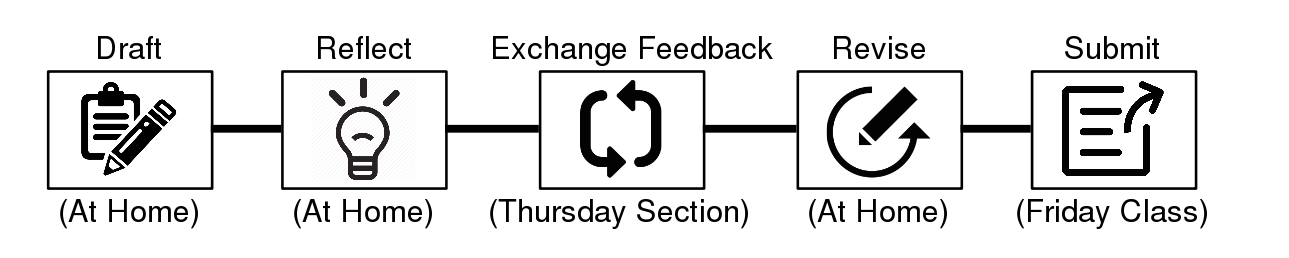
\includegraphics[scale=0.7]{flow_chart.pdf}\end{center}

\textbf{Important note:} This week, you MUST type your response to at least one of the PAR problems in \LaTeX{}.

\textit{\LaTeX{} note:} To produce the $\R$ symbol, import the package \verb!amsfonts! and use the command \verb!\mathbb{R}!.

\bigskip

\textbf{Problem Statement}

A \textbf{transformation} is a rule that turns input vectors into output vectors.  For example, the following transformations turn vectors in $\R^2$ into other vectors in $\R^2$:
\begin{itemize}
	\item Multiply the first component by 2
	\item Add 1 to the second component
\end{itemize}

A special kind of transformation is the transformation associated to a matrix $A$.  This transformation turns the vector $\vec{v}$ into $A\vec{v}$.

\begin{enumerate}
	
	\item For each of the following matrices, describe the associated transformation in words.  Explain how you got your answer.
	\begin{enumerate}
		\item $\mat{1 & 0 \\ 0 & 2}$
		\item $\mat{1 & 1 \\ 1 & 0}$
	\end{enumerate}
	
	\item For each of the following transformations from $\R^2$ to $\R^2$, either find a matrix that gives the transformation, or explain why there is no such matrix.
	\begin{enumerate}
		\item Flip the sign of the first component.
		\item Add 1 to the second component.
		\item Rotate the vector counterclockwise (around the origin) by 90 degrees.
	\end{enumerate}
	
	\item Let $A = \mat{1 & 0 & 0 \\ 0 & 1 & 0}$, and $B = \mat{1 & 0 & 0 \\ 0 & 1 & 0 \\ 0 & 0 & 0}$. Describe the transformations associated to $A$ and $B$. Make sure to include a description of their domain and range as well as what the transformations do.  Are both transformations the same? Explain how they are or aren't.
	
	\item We often like to think of a vector in $\R^2$ as actually sitting in a plane in $\R^3$.  Come up with a matrix whose corresponding transformation takes vectors in $\R^2$ and ``sets them down'' in $\R^3$.  How many such matrices are there?  Explain.
\end{enumerate}



\vspace{0.5in}

\begin{center}{\Large{\textbf{Reflection\\}}}

Turn the page and check off the icons that you think you did well; circle icons that you want feedback on. \end{center}

\newpage

\begin{center}{\Large{\textbf{Feedback Provided By: \rule{6cm}{0.5pt}}}}\end{center}

\begin{tabular*}{\textwidth}{@{\extracolsep{\fill}}l c r}
\textbf{Suggestions} & Communication & \textbf{Strengths}  \\
\hline
\end{tabular*}
\begin{center}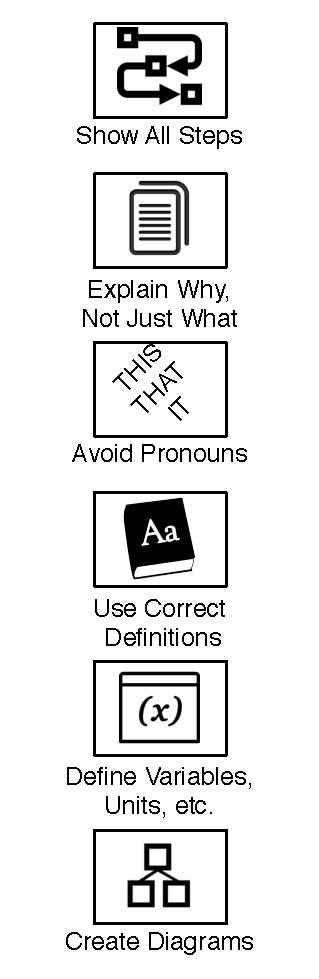
\includegraphics[scale=0.7]{communication.pdf}\end{center}

\begin{tabular*}{\textwidth}{@{\extracolsep{\fill}}l c r}
\textbf{Suggestions} & Accuracy & \textbf{Strengths}  \\
\hline
\end{tabular*}

\begin{center}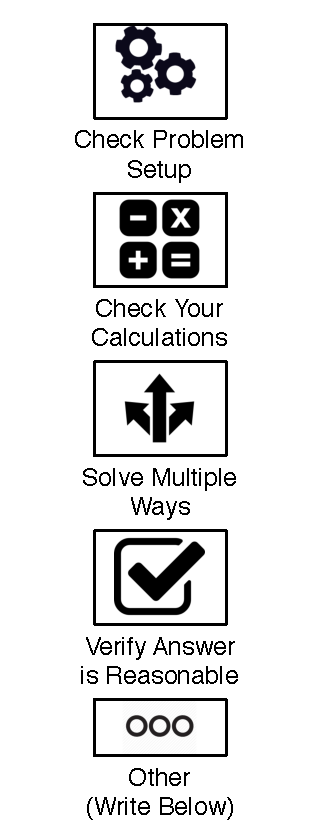
\includegraphics[scale=0.7]{accuracy.pdf}\end{center}




\end{document}
